%--------------------------------------------------------------------
%--------------------------------------------------------------------
% Formato para los talleres del curso de Métodos Computacionales
% Universidad de los Andes
% 2015, curso de vacaciones
%--------------------------------------------------------------------
%--------------------------------------------------------------------

\documentclass[11pt,letterpaper]{exam}
\usepackage[utf8]{inputenc}
\usepackage[spanish]{babel}
\usepackage{graphicx}
\usepackage{mdframed}
\usepackage{tabularx}
\usepackage[absolute]{textpos} % Para poner una imagen en posiciones arbitrarias
\usepackage{multirow}
\mdfdefinestyle{mystyle}{leftmargin=1cm,rightmargin=1cm,linecolor=red}
\usepackage{float}
\usepackage{hyperref}
\decimalpoint

\newcommand{\base}[1]{\underline{\hspace{#1}}}
\boxedpoints
\pointname{ pt}
%\extrawidth{0.75in}
%\extrafootheight{-0.5in}
\extraheadheight{-0.15in}
\hypersetup{%
  colorlinks=true,% hyperlinks will be coloured
  urlcolor=blue
}

%\noprintanswers
%\printanswers
\renewcommand{\solutiontitle}{}
\SolutionEmphasis{\color{blue}}

\usepackage{upquote,textcomp}
\newcommand\upquote[1]{\textquotesingle#1\textquotesingle} % To fix straight quotes in verbatim

\begin{document}
\begin{center}
{\Large Métodos Computacionales} \\
Tarea 4 - DFT \\
Junio de 2015
\end{center}

\begin{textblock*}{40mm}(10mm,20mm)
  
\includegraphics[width=3cm]{logoUniandes.png}
\end{textblock*}

\begin{textblock*}{40mm}(164mm,20mm)
  
\includegraphics[width=3cm]{logoUniandes.png}
\end{textblock*}

\vspace{0.5cm}

La solución a este taller debe presentarse en un {\it notebook} llamado \verb+HW4.ipynb+ y debe cargarse a su repositorio en GitHub en la carpeta /MC/Tareas/HW4/. Es requisito que en todo lo hecho se pongan comentarios que expliquen lo que se está haciendo. La fecha límite para hacer un commit es el \textbf{jueves 25 de junio a las 23:59}. Puede trabajar en parejas.

\vspace{0.5cm}

\begin{questions}
 
\question (Difracción de Fraunhofer) El patrón de difracción producido producido por una apertura en el régimen de Fraunhofer ( ver \href{http://www.google.com}{Born \& Wolf, Principles of Optics} capítulo 8 ) puede encontrarse a través de una integral de Fourier y aproximarse numéricamente a través de una DFT. En este ejercicio exploramos los patrones de difracción producidos por aperturas de diferentes formas usando diferentes {\it pupil functions} (ver Born. pág 385). Imaginamos que las aperturas se encuentran en el centro de una placa de lado $L=1 \,\textrm{u}$ y la representamos por medio de un array cuadrado de 1024 elementos en cada dirección. 

\begin{parts}

\part[20] Comenzando con un array de ceros de lado 1024 manipularlo con ciclos o usando {\it slice notation} para dejar todo en cero excepto elementos en un cuadrado de lado 32 en el centro.

\part[20] Calcular la DFT del array resultante y aplicar sobre él la función  \href{http://docs.scipy.org/doc/scipy-0.14.0/reference/generated/scipy.fftpack.fftshift.html}{fftshift}, esto hace un cambio de coordenadas que arroja el patrón de interferencia esperado. De lo resultante tomar del centro un cuadrado de lado 200 y producir una imagen del logaritmo del módulo al cuadrado usando \verb+imshow+ con la representación de la apertura a su izquierda.

\begin{center}
	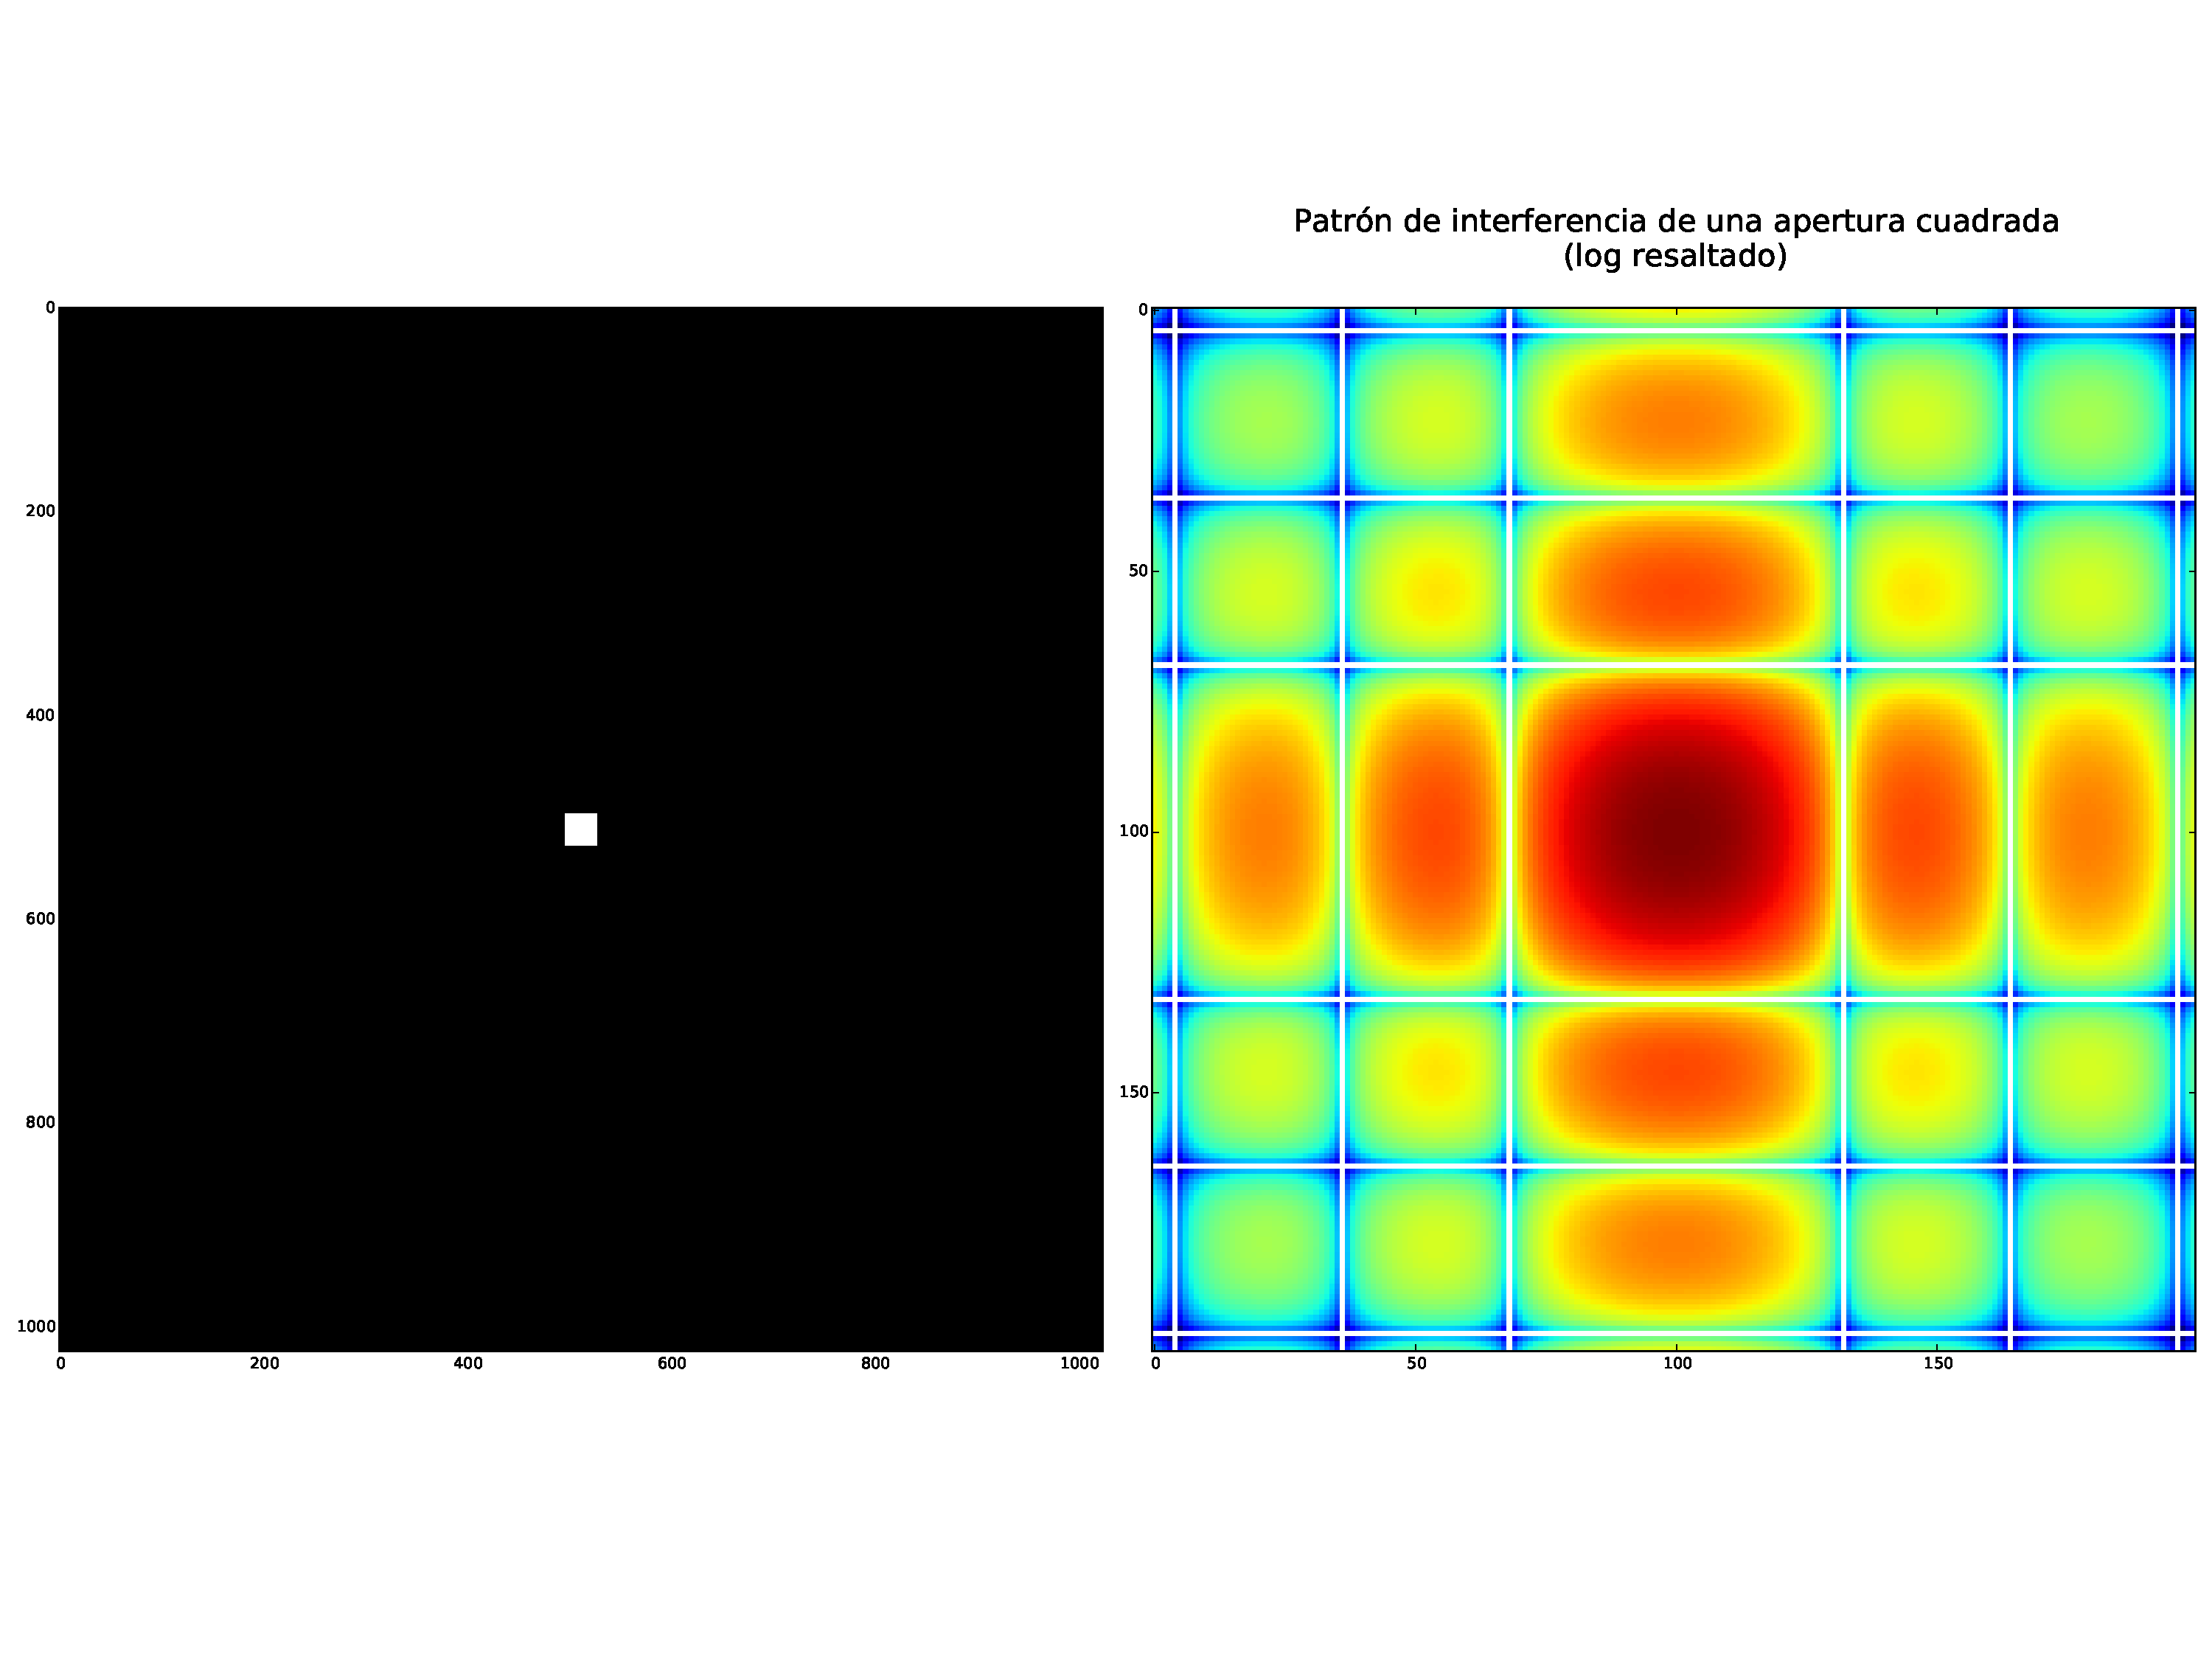
\includegraphics[width=0.9\textwidth]{./squareaperture.pdf}
\end{center}

\part[20] Repita los dos anteriores literales para una doble rendija cada una de ellas con una altura de 200, grosor 20 y con sus ejes en las columnas 460 y 564. Esta vez tome un cuadrado de lado 128 para la gráfica del patrón de difracción y no resalte con \verb+log+.

\begin{center}
	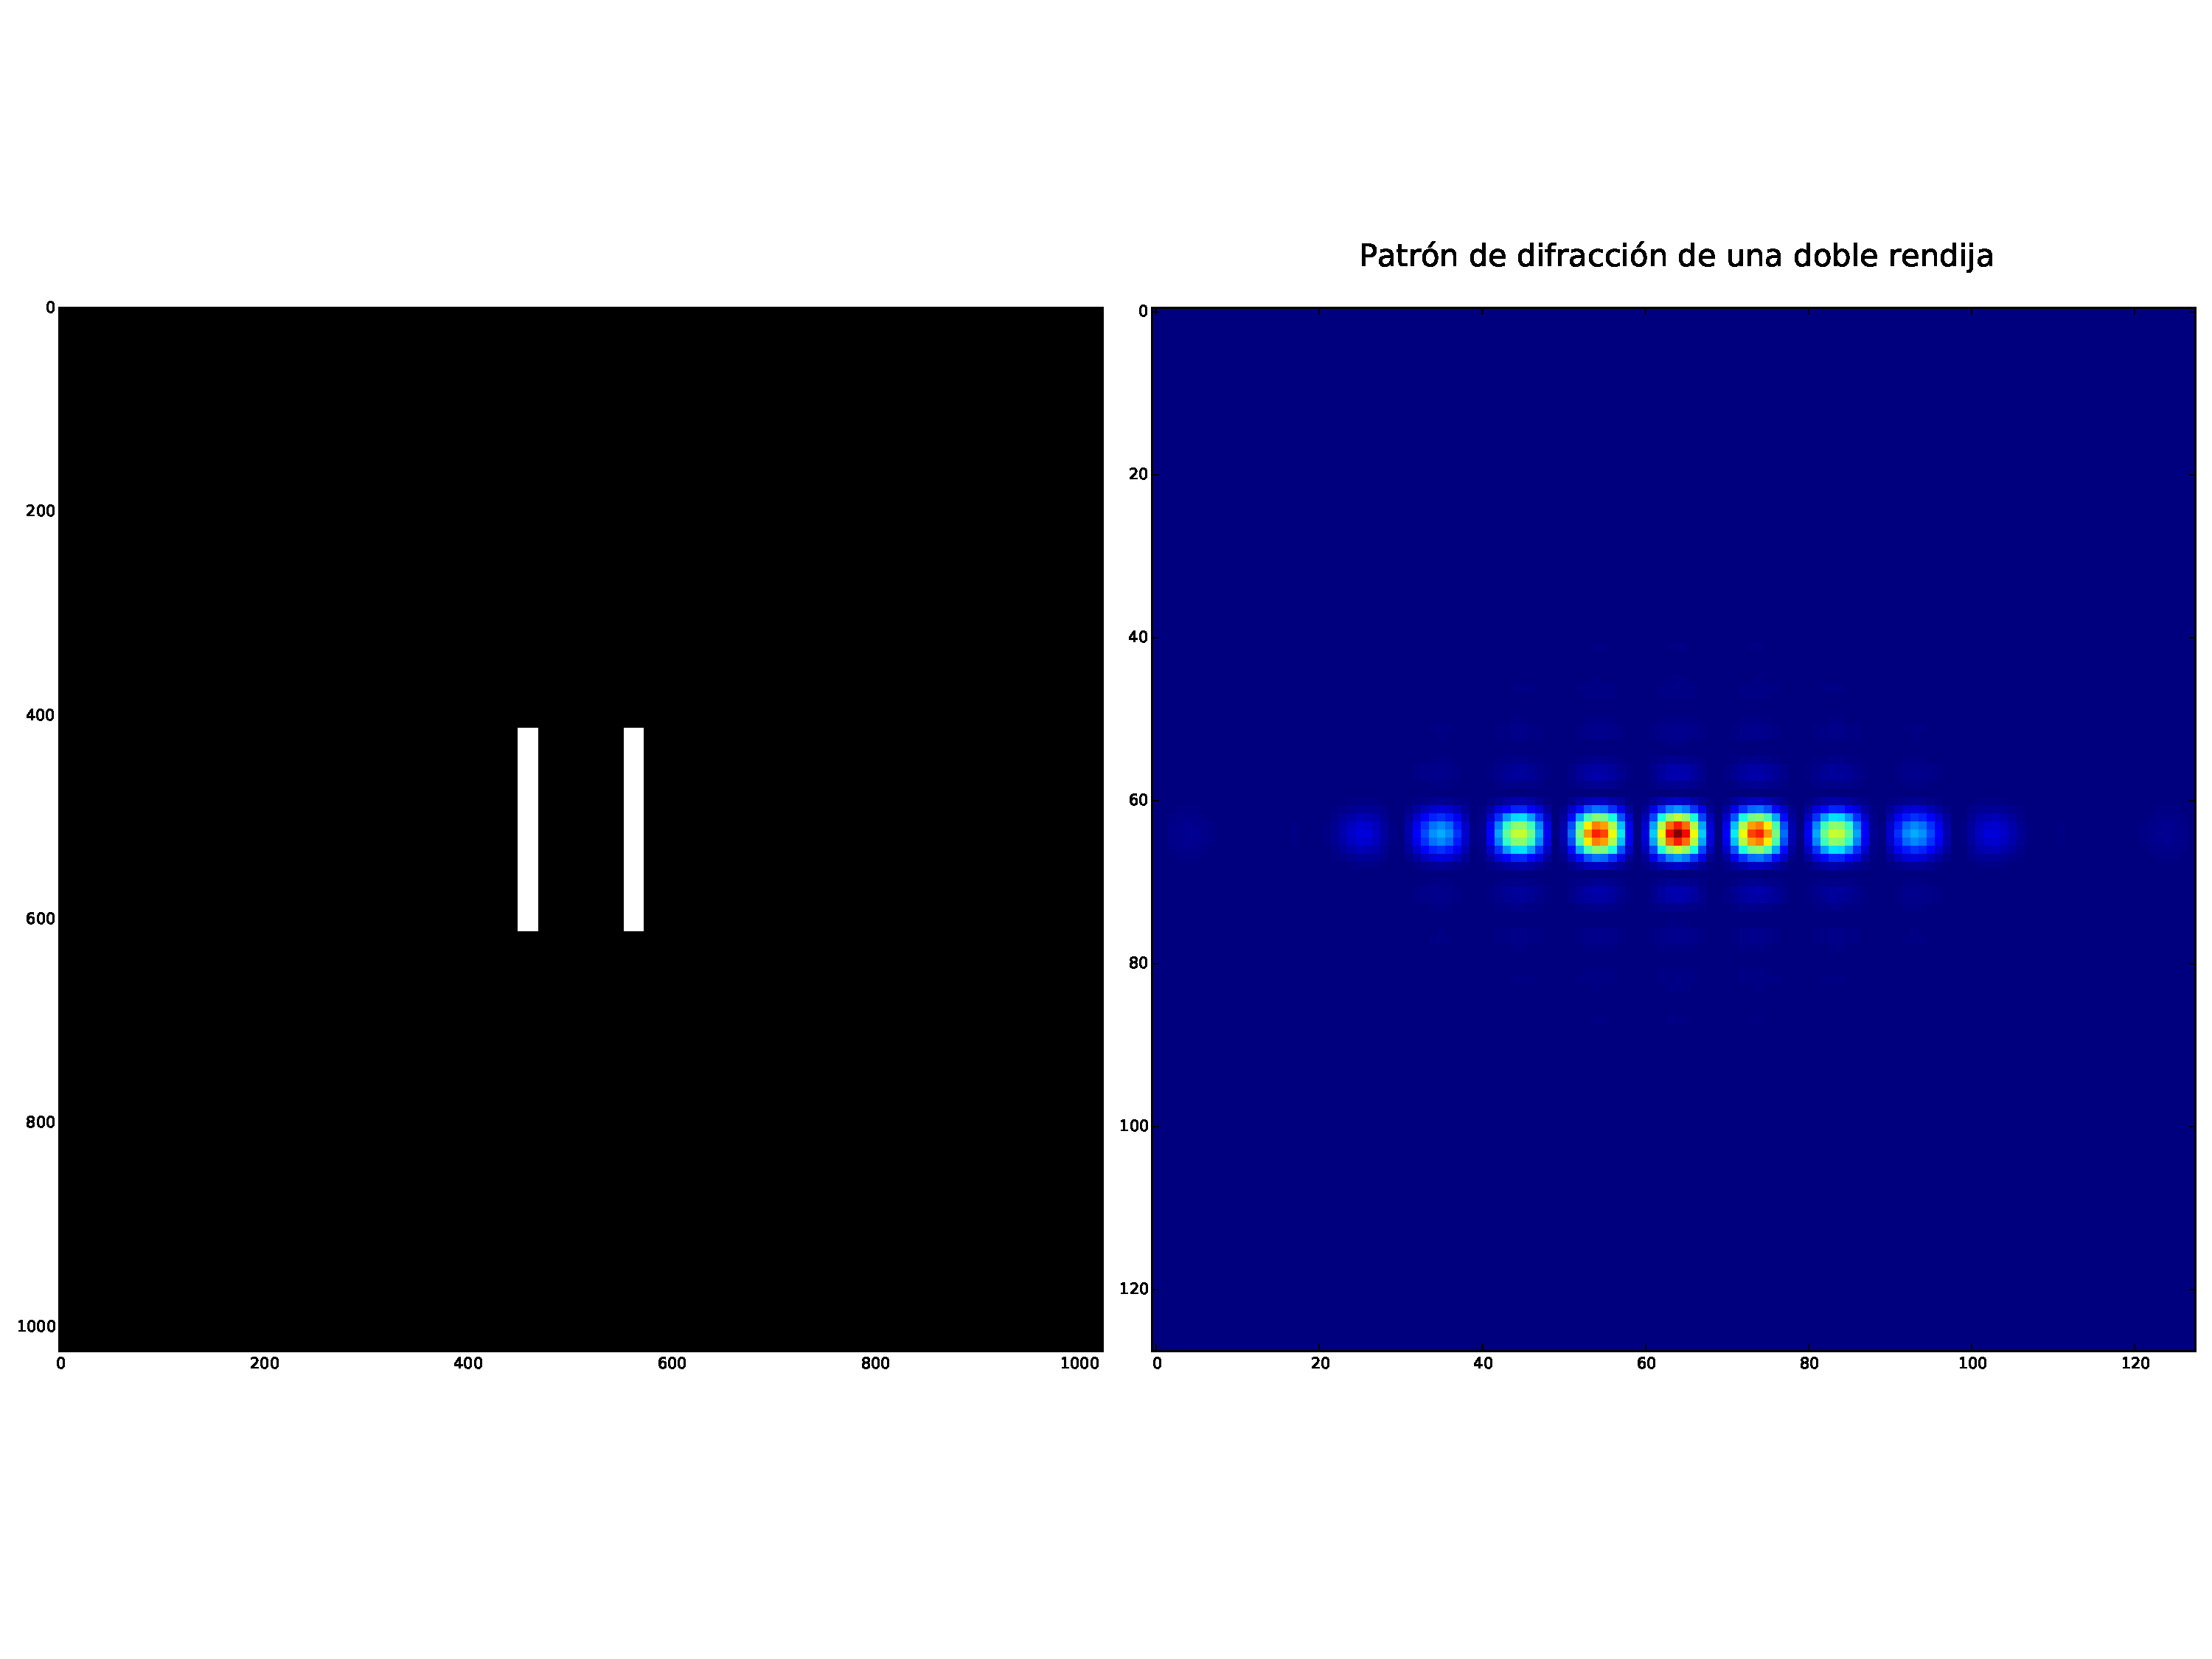
\includegraphics[width=0.9\textwidth]{./twoslits.pdf}
\end{center}

\part[20] Ahora hágalo para una apertura circular de radio $0.01\,\textrm{u}$ y además de lo anterior tome ahora la fila central y tomando como abscisas \verb+2*pi*radio/1.*linspace(-512,512,1024)+ reproduzca la gráfica mostrada abajo; las abscisas están así elegidas para hacer comparable nuestro resultado con lo mostrado en la pág. 396 de los {\it Principles} de Born. $I_0$ es la amplitud máxima.

\begin{center}
	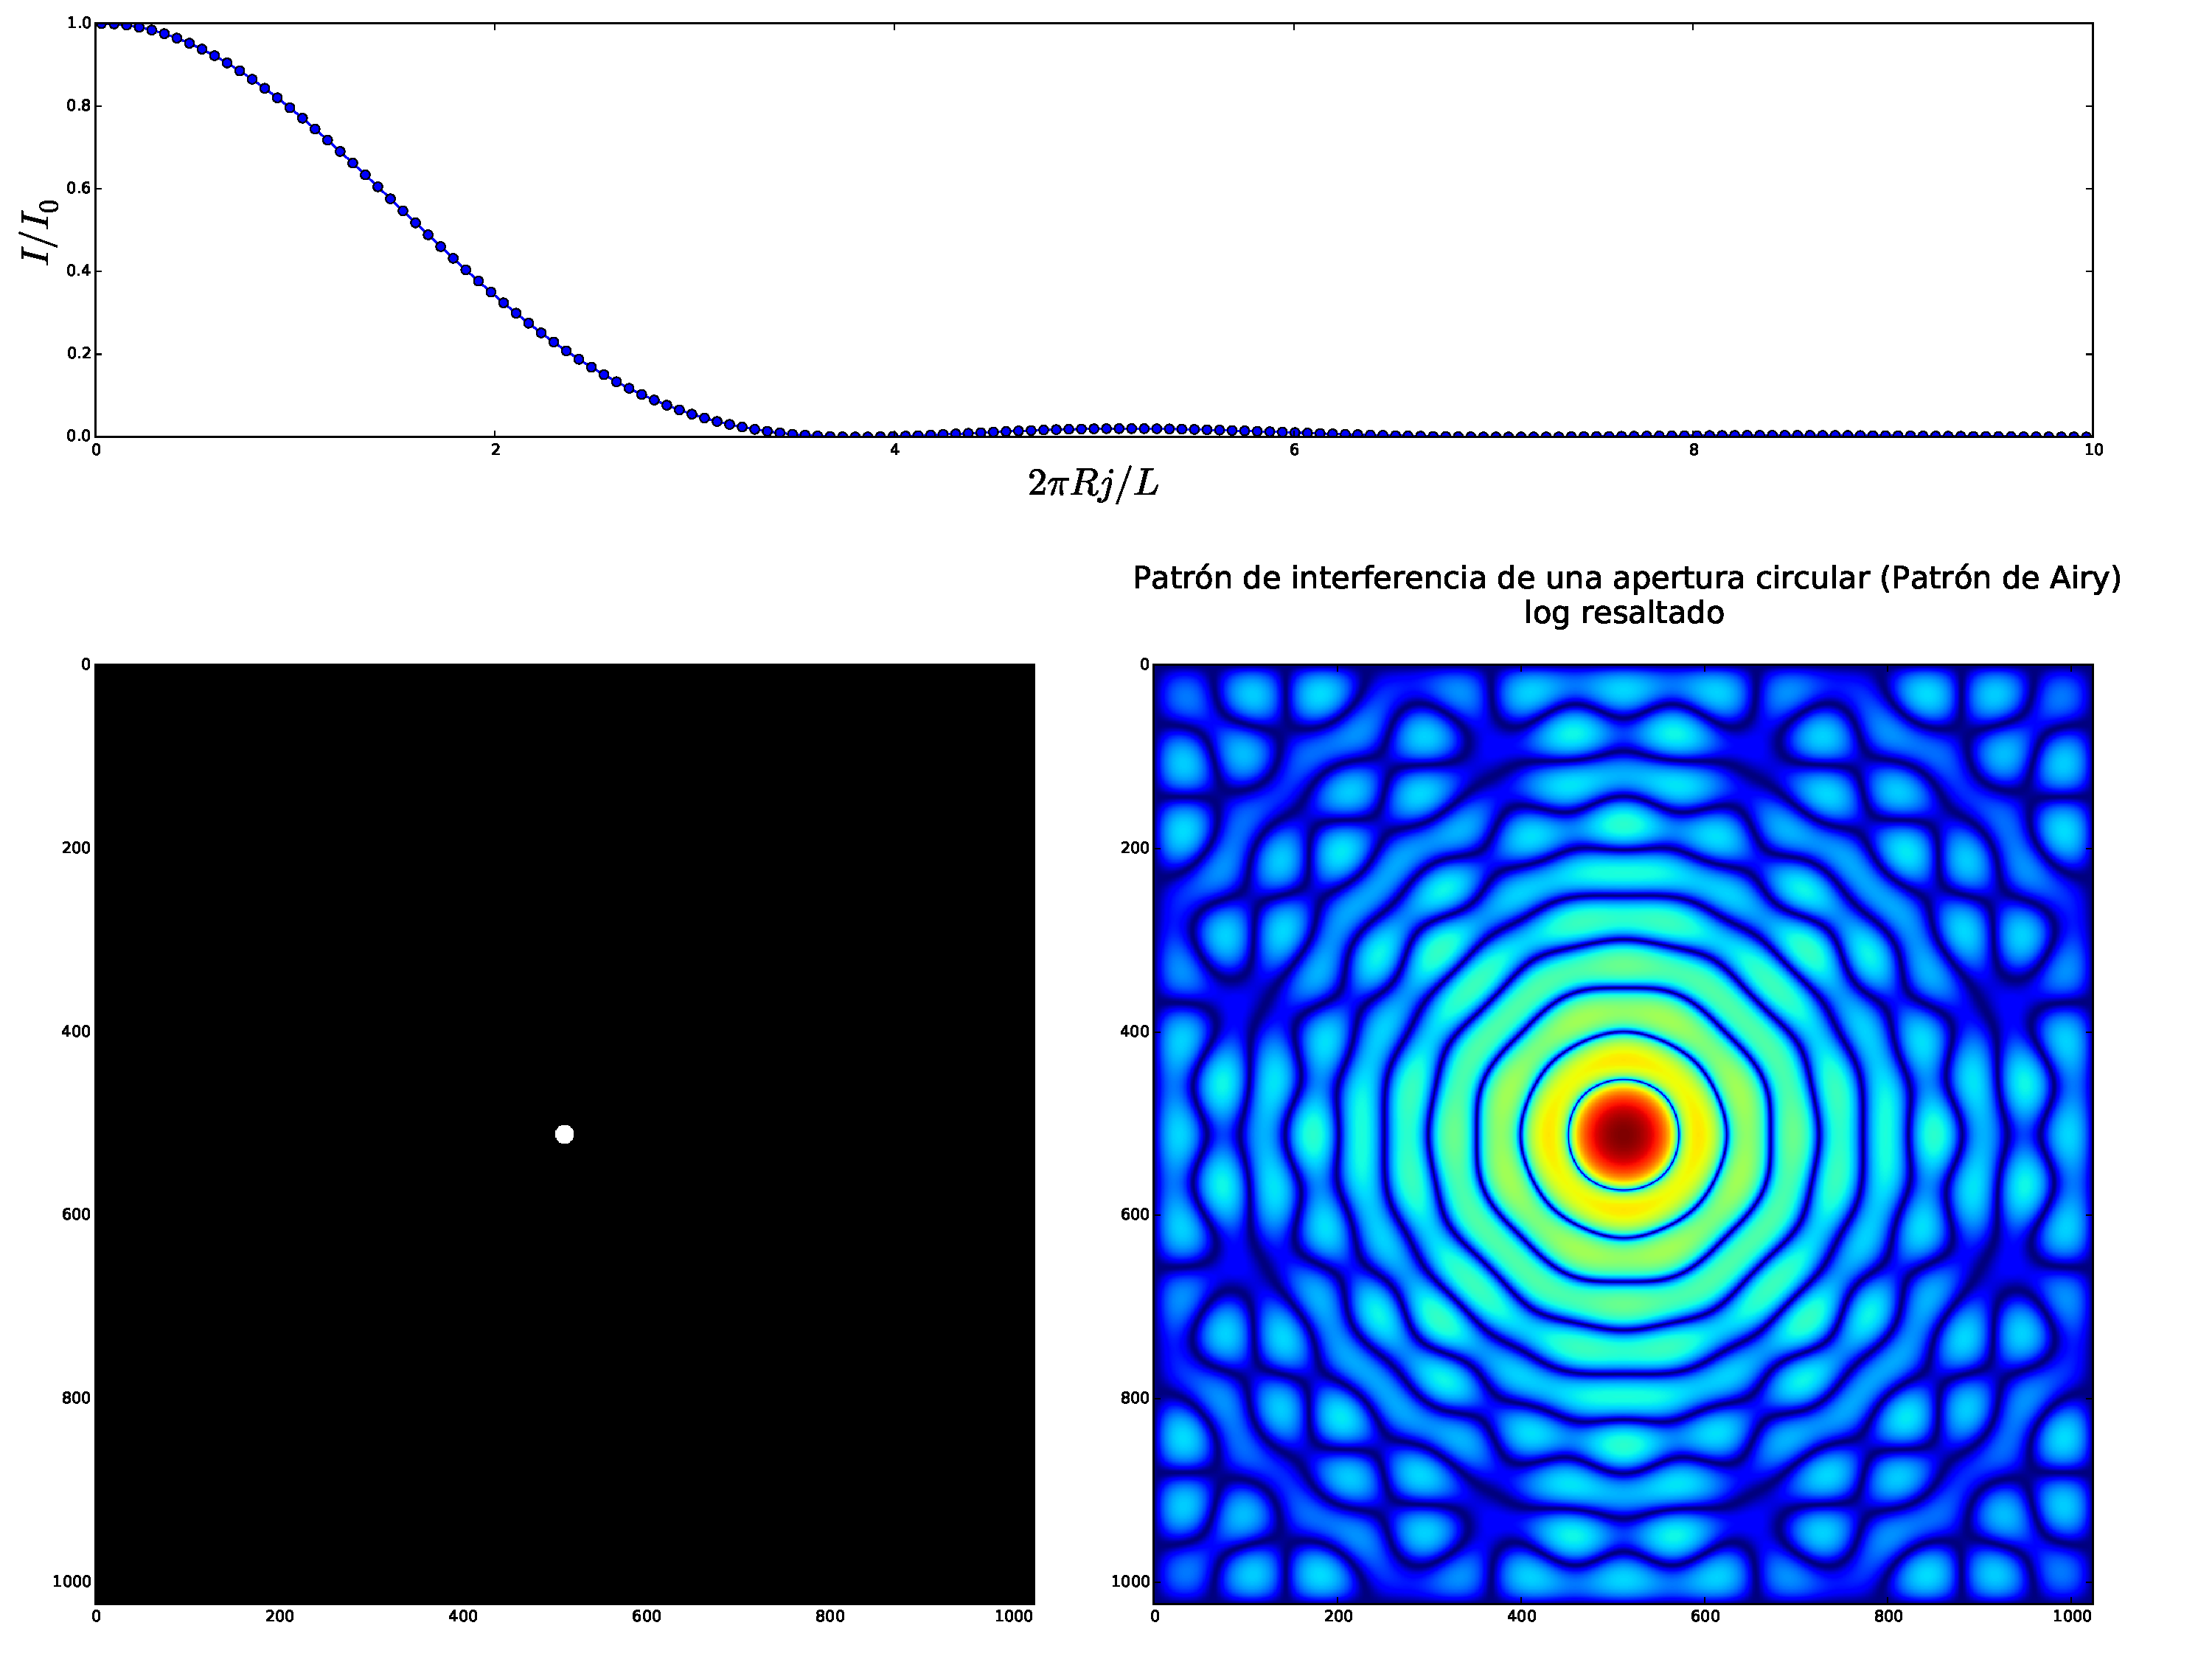
\includegraphics[width=0.95\textwidth]{./Airy.pdf}
\end{center}

\part[20] Usando las mismas ordenadas y abscisas del anterior literal calcular los máximos y mínimos entre $0.$ y $12.0$. Al hacerlo {\bf{debe}} utilizar interpolación en algún momento. Compare sus resultados con la tabla mostrada en la pág. 397 de los {\it Principles}:

\begin{center}
	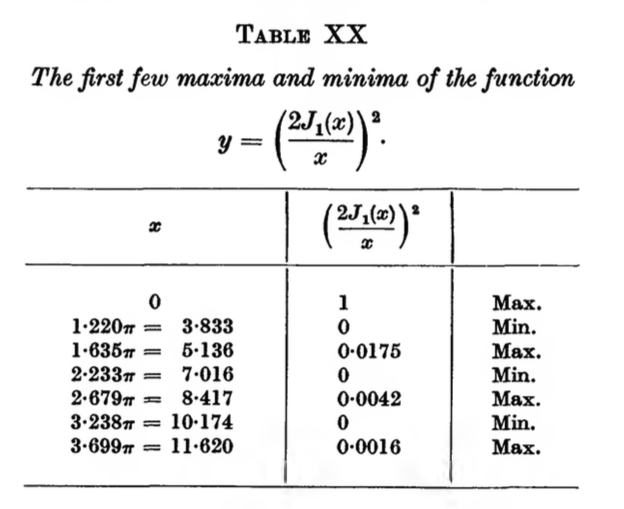
\includegraphics[width=0.6\textwidth]{./BornTabla.png}
\end{center}
\end{parts}
\end{questions}

\newpage
COMENTARIOS:

\begin{itemize}
	\item Si al aplicar \verb+log+ encuentra una advertencia sobre el intento de hacer \verb+log(0)+ sume 1 a todo antes de usarlo.
	\item El panel para la apertura circular se hizo con la ayuda de \verb+subplot2grid+:
\end{itemize}

\begin{verbatim}
             plt.figure(figsize=(20,15))
             plt.subplot2grid((3,2),(0,0),colspan=2,rowspan=1)
             
             ...
             
             plt.subplot2grid((3,2),(1,0),rowspan=2)
             
             ...
             
             plt.subplot2grid((3,2),(1,1),rowspan=2)
             
             ...
             
             plt.tight_layout()
             plt.show()
\end{verbatim}

\end{document}
